\chapter{Introduction}\label{ch:intro}

The 21st century is flushed with a massive amount of texts and documents. Every day there are new articles, news, documentation and reports packed full of information. For this reason, a new discipline arose out of this. Knowledge is nowadays accessible everywhere and immediately, but consumption takes way too much time. Websites like \textit{https://www.blinkist.com/de} provide their costumer's text summarizations of different kinds of books readable in 15-30 minutes. This is an exciting way to save time, but still, this summarization is done by hand. Artificial Intelligence researchers continuously provide knowledge to the public to summarize text with computer algorithms. The first approaches of automatic text summarization were grammatically wrong and reading grammatically broken summarizations is tiring for the most people. Deep Learning changed the game entirely, because algorithms are now feasible enough to summarize texts as good as humans do.

\section{Structure of the thesis}
The aim of my thesis is to survey the current state of the art in text generation, especially on the focus of text summarization. The development into the state of the art neural text summarization had a huge impact on the readability for the human. For readers who are not familiar with machine learning in general, I will provide a zoom-in introduction from artificial intelligence in general into the tiny sub field text summarization. My approach is feed-forward from the definition of machine learning, deeper into the natural language processing field, further into the text generation field and within that, I focus on the text summarization part in chapter 1 - Introduction. New research and state of the art results in some natural language processing fields often lead to improvements across other related disciplines in machine learning and natural language processing, because algorithms are sometimes usable vice-versa. For this reason, I provide the most crucial text generation historical achievements in combination with the latest text summarization results, because both topics intersect in many aspects. The crucial concept of historical and modern approaches to summarize and generate text are introduced in chapter 2 - An evolutionary view on the State of the Art. 
To illustrate the basic workflow of a text summarizing system, I programmed a prototype. The concept, development and evaluation of this summarizer are located in chapter 4 - Prototype, but it requires prior knowledge to fully understand the mechanism from the input to the output. Finally in the last chapter I will discuss further improvements for my prototype and a brief discussing of future of text generation.

\section{Machine Learning}
In the last decade, Machine Learning (ML) is increasingly finding its way into businesses and society. Many websites and businesses use Machine Learning techniques to improve user and customer experience. The phrase \textit{Machine Learning} was initially introduced in 1952 by Arthur Samuel. He developed a computer program for playing the game checkers in the 1950s. Samuel's model was based on a model of brain cell interaction by Donald Hebb from his book called \textit{The Organization of Behavior} published in 1949. Hebb's book introduces theories on neuron excitement and neural communication. Figure \ref{neuron} illustrates a mathematical approximation of the human's brain cell in the form of a \textit{artifical} neuron. Nowadays, this brain-neuron based model is mostly declared to be not close enough to reality [Andrew Ng, deeplearning.ai], because the structure of a brain's neuron is far more complicated than the illustration in figure \ref{neuron} suggests. Nevertheless, it provides an excellent entry point for this research field in my opinion. 

\begin{figure}
  \begin{center}
  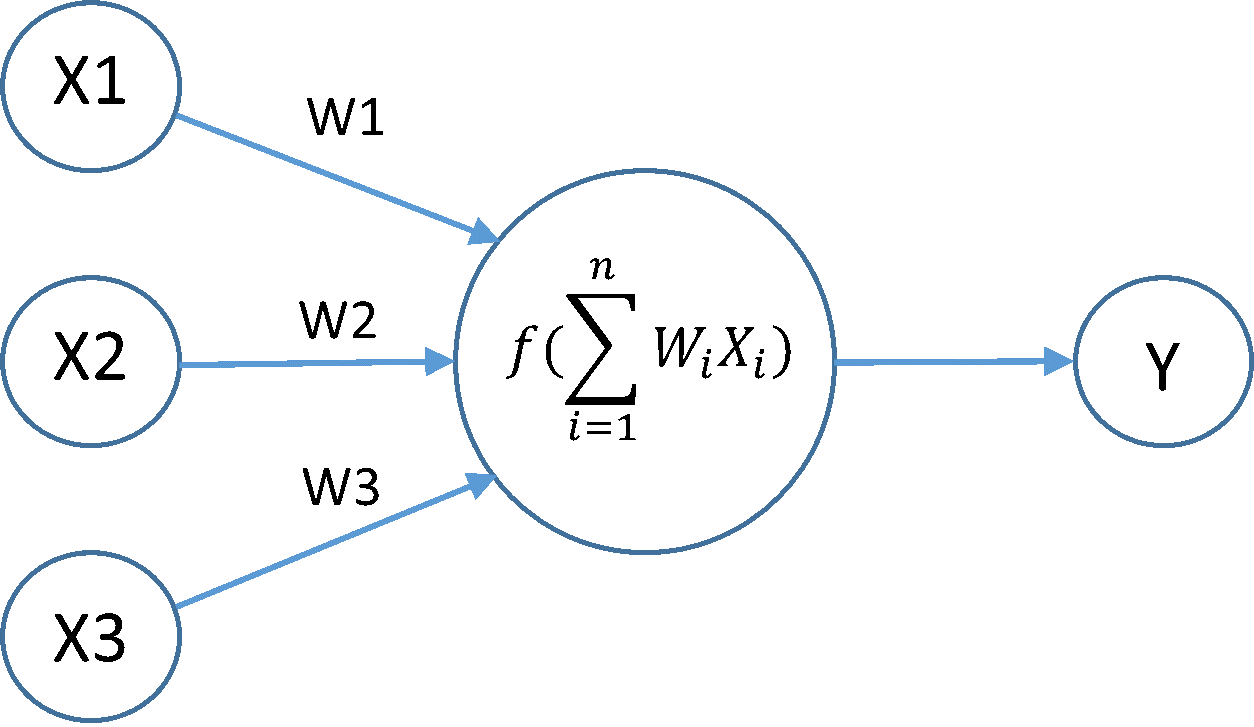
\includegraphics[width=3.5in]{photos/neuron}\\
  \caption{A simple Neuron with 3 inputs and 1 output \cite{neuron}}\label{neuron}
  \end{center}
\end{figure}
 
The roots of Neural Networks (NN) lie down almost 80 years ago in 1943 when \textbf{McCulloch-Pitts} \cite{NN} compared for the first time neural networks with the structure of the human brain. The range in which Neural Networks (in the year 2020) apply to modern technologies is wide. Some disciplines have only been created due to the invention of Neural Networks, because they solve existing and new problems more effectively and efficiently than previously used algorithms. Many frequently held conferences around the globe prove continuous evidence of the successes of Neural Networks. Among those various disciplines counts for example \textit{Pattern recognition} with Convolutional Neural Networks (CNN) \cite{cnn}. Convolutional Neural Networks are one of the many special building blocks of the neural network. Every building block aims to solve a different task. For example, Pattern recognition uses different layers (building blocks) in its neural network than text summarization, because the input for Pattern recognition neural networks is often a picture consisting of e.g., 32x32 pixels. In contrast, the input for the text summarization is e.g., a 1000 word long text.  

A widely known entry challenge into pattern recognition is the \textit{CIFAR-10} dataset \cite{cifar}. It consists of 50.000 images divided into ten classes of different objects and animals like cats and cars (5000 images of cats, 5000 images or cars, ...). Classification algorithms try now to predict a class for the input image as precisely as possible. Many amateurs \cite{tim} and experts annually attempt to show their latest results in beating the former best accuracy. 

Natural Language Processing is one of the various sub-fields of Machine Learning. Strictly speaking, it is a multidisciplinary field consisting of Artificial Intelligence (AI) and computational linguistics. Natural Language Processing is dedicated to understand and process the interactions between human (natural) language and computers. Natural Language Processing is a broad term and can be applied to many different tasks, such as: 

\begin{itemize}
\item \textbf{Sentiment Analysis}, e.g. Google Reviews on Restaurants
\item \textbf{Machine Translation}, e.g. Google Translator
\item \textbf{Speech Recognition}, e.g. Siri from Apples IPhone
\item \textbf{Text Generation (Neural Text Generation [\textit{NTG}])}, e.g. Text Summarization
\item \textbf{Chat Bots}, e.g. Shopping Websites
\end{itemize}

\textbf{Deep Learning} is not an absolute definition. Many top researchers define it in a very different way. In general, Deep Learning allows building more complex neural networks, which are capable of detecting better and more correlation in data. Figure \ref{ai} shows the zoom-in from AI to Deep Learning. Therefore Deep Learning can be seen as a method in Machine Learning, not to mix up with Natural Language processing, which can make use of Deep Learning techniques, but it is not required to use it.

\begin{figure}
	\begin{center}
		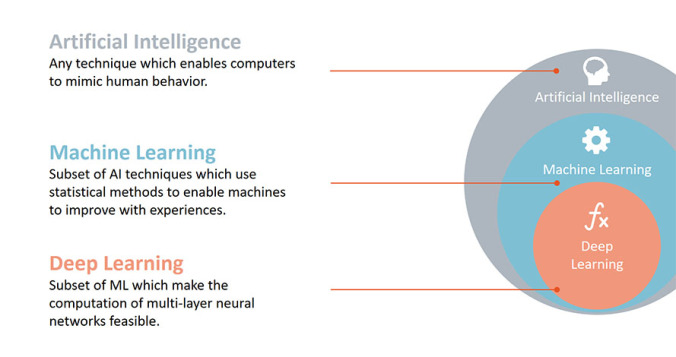
\includegraphics[width=5.5in]{photos/ai_ml_dl.jpg}\\
		\caption{Zoom into Artificial Intelligence from \textit{https://rapidminer.com/blog/artificial-intelligence-machine-learning-deep-learning/}}\label{ai}
	\end{center}
\end{figure}

All of these tasks require many steps to function correctly. In the broadest sense, there is always an Input and an Output, which are shown in Table \ref{tab:nlp_table}.

\begin{center} 
	\begin{tabular}{ |p{3cm}||p{3cm}|p{3cm}|p{3cm}|}
		\hline
		\multicolumn{4}{|c|}{\textbf{Example components of Input - Output systems}}\\ \hline\hline
		&Speech &Text &Images \\ \hline
		Input &Speech &Text &Image \\
		Analysis &Recognition  &Recognition     &Recognition \\ \hline \hline
		Output &Generation &\cellcolor[HTML]{F3E687}Generation &Generation \\
		Synthesis &of Speech & \cellcolor[HTML]{F3E687}of Text &of Images \\ \hline \hline
		Processing &NLP &\cellcolor[HTML]{7ebfd3}NLP &CNN \\
		method &method  &\cellcolor[HTML]{7ebfd3}method     &Building Blocks \\ \hline
	\end{tabular}
	\captionof{table}{A closer look into Input Output systems with the focus on Text Generation}
	\label{tab:nlp_table}
\end{center}

\begin{center} 
	\begin{tabular}{ |p{3cm}||p{3cm}|p{3cm}|p{3cm}|}
		\hline
		\multicolumn{4}{|c|}{\textbf{Examples of Natural Language Processing systems}}\\ \hline\hline
		&Speech &Text &Text \\ \hline
		Input &Siri &Read in &Read in \\
		Analysis &listens  &document     &document \\ \hline \hline
		Output &Siri &\cellcolor[HTML]{F3E687}Generate &Generate \\
		Synthesis &answers & \cellcolor[HTML]{F3E687}Summary &sentiment \\ \hline
	\end{tabular}
	\captionof{table}{Examples for three different NLP tasks}
	\label{tab:nlp_table2}
\end{center}

It shows that Text Generation is the \textbf{output part} of a \textbf{Natural Language Processing} model. Data is collected through various sources, e.g. images, videos or speech, then it is further processed and generates the desired output. Useful examples are shown in Table \ref{tab:nlp_table2}.

For this Bachelor thesis, the focus is on the output part of a Natural Language Processing system. More specifically, the text summarization which inputs text as shown in Table \ref{tab:nlp_table} and \ref{tab:nlp_table2} and outputs the summary is what I treat in my work. Text generation is therefore generally the output-synthesis part of an input-output NLP system.

However, what defines a summarization and what defines a good summarization? The literature points out multiple different definitions. One definition proposes that the summary of a document is the process of distilling the essential information from a source (or sources) to produce an abridged version for a particular user (or users) and task (or tasks) \cite{def}. Its objective is to give information and provide classified access to the source documents. Summarization is an automatic task when it is generated by software or an algorithm.

Another term for Text Generation is  \textit{Language Modelling}, because text generators use the words of a language and grammar as input for the model. In the past five years, primarily two approaches were used for modeling a Natural Language Processing system, namely the \textbf{rule-based} system and the \textbf{template-based} system (Figure \ref{rules_based}) \cite{NTG2}. Today neural end-to-end systems are \textit{state-of-the-art} \cite{End_to_End}. These systems offer more flexibility and scale with proportionately better results, and less data is required because of the increased complexity. These systems are called neural, because they make use of \textbf{Deep Learning} Neural Networks.
A significant disadvantage is that the necessary computing power has increased exponentially. This computing power requires a strong server and most language models are trained on a very large scale. This can most commonly not be achieved by a single person at home, except if one rents for example a strong server from the \textit{Amazon Web Services}. The computational requirement rose in such a way, because of the more profound and deeper neural networks nowadays. However, this leads to a complex problem because it becomes more and more challenging to understand the decisions of the neural network. The neural network is still, to a large extent, a \textit{black box}. Nevertheless, especially in NLP, it gives surprisingly good results. The neural network models for text processing are difficult to understand, so nowadays, compromises between rule-based systems still have to be made, and hybrid systems are most commonly in use. 


\begin{figure}
  \begin{center}
  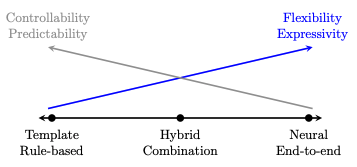
\includegraphics[width=3.5in]{photos/rule_based}\\
  \caption{Rule-Based vs. Neural-Text-Generations System \cite{NTG2}, Page 4}\label{rules_based}
  \end{center}
\end{figure}

When Neural end-to-end systems are used, Text Generation is often referred to as Neural Text Generation (NTG). More examples for Neural Text Generators as output synthetical component are:

\begin{itemize}
\item Speech recording and conversion to text
\item Conversation systems e.g. chatbots
\item Neural Text summary
\item Caption generation of Images
\end{itemize} 

In order to train language models properly, Deep Learning (DL) algorithms teach the model the probabilities of occurring words with respect to the preceding words. There are several approaches to achieve this goal. Language models can be trained on the level of words, whole sentences, or even whole paragraphs. The granularity in which the training takes place is called \textit{n-grams}, where \textit{n} represents the number of preceding words. 


\section{Case study of an Automatic Text Summarization System (ATS)}\label{ss:case}

As a human, creating a good summary of a text requires that the person understood the text well. The text needs to be understood so well, that the person can summarize the essence of the text in such a way, that it shortens the original document to a minimum down without cutting out important information. However, after a while, a person is most likely to summarize the same text differently than one month ago. Due to this circumstance, the summarization task tends to be challenging to automate. Depending on what kind of summary is needed, the texts must be processed differently into different fragments with multiple relevances for each fragment. A crucial role is also the coherence of a text. Different applications of text summarizations are:

\begin{itemize}
	\item Web Page Summarization
	\item Reports or Meetings
	\item Opinion Summarizations
	\item Scientific Research Papers
	\item News Headlines
\end{itemize}


\textbf{Google News Headline Summarization}

Google has its own news section on this link \textit{https://news.google.com}. Google News automatically generates the news headlines for multi-language news articles \cite{google}. Google proposes that for people to digest a large amount of daily information better, they created the long-term goal at the \textit{Google Brain} department to summarize news articles and their headlines as pleasant as possible. The search engine Google is known for its accurate and many search results when using this engine. Google does the same for Google News. Google scrapes news articles all over the world, automatically summarizes it, and out of that, it generates the headline of the summarized news article out of it \cite{google}. 
For achieving their state of the art results, Google makes use of a Deep Learning technique called \textit{sequence-to-sequence} learning, which will be explained in Section \ref{ss:seq2seq}. Table \ref{tab:google} shows an example for generated headlines of a summarization. Due to the structure of a news article, a good headline summary requires most likely only the first few sentences of an article.  

Many examples from this thesis will be conducted from the perspective of a news article to keep it uniform, whether a long text will be summarized to a shorter text or only one or two sentences for a headline will be extracted and summarized from an article. 


\begin{table}[]
	\begin{tabular}{|c|c|l}
		\cline{1-2}
		\textbf{Input: Article 1st sentence}                                                                                                                                                                                                                                 & \textbf{Model-written headline}                                                                 &  \\ \cline{1-2}
		\begin{tabular}[c]{@{}c@{}}metro-goldwyn-mayer reported a third-quarter \\ net loss of dlrs 16 million due mainly to the \\ effect of accounting rules adopted this year\end{tabular}                                                                                & \begin{tabular}[c]{@{}c@{}}mgm reports 16 million \\ net loss on higher revenue\end{tabular}    &  \\ \cline{1-2}
		\begin{tabular}[c]{@{}c@{}}starting from july 1, the island province of hainan in \\ southern china will implement strict market \\ access control on all incoming livestock and animal \\ products to prevent the possible spread of epidemic diseases\end{tabular} & \begin{tabular}[c]{@{}c@{}}hainan to curb \\ spread of diseases\end{tabular}                    &  \\ \cline{1-2}
		\begin{tabular}[c]{@{}c@{}}australian wine exports hit a record 52.1 million liters\\  worth 260 million dollars (143 million us) in september, \\ the government statistics office reported on monday\end{tabular}                                                  & \begin{tabular}[c]{@{}c@{}}australian wine exports\\  hit record high in september\end{tabular} &  \\ \cline{1-2}
	\end{tabular}
	\captionof{table}{ The first column shows the first sentence of a news article which is the model input, and the second column shows what headline the model has written \cite{google}.} 
	\label{tab:google}
\end{table}


